% Dokumenten Setup
\documentclass[
  a4paper,
  12pt,
  titlepage,	
  ngerman,
  footheight=15pt,
  headheight=15pt,
  oneside
]{scrbook}

% Hier bitte nur bei gegebener LaTeX Erfahrung Änderungen vornehmen.
%Packages
\usepackage{babel}
\usepackage[parfill]{parskip}
\usepackage{mathptmx} 
\usepackage[utf8]{inputenc}
\usepackage[T1]{fontenc}
\usepackage[intlimits]{amsmath}
\usepackage{amssymb}
\usepackage{url}
\usepackage{subcaption}
\usepackage{geometry}
\usepackage{multirow}
\usepackage{booktabs}
\usepackage[page]{totalcount}
\usepackage[dvipsnames,svgnames,x11names,table]{xcolor}
\usepackage{scrlayer-scrpage}
\usepackage[parfill]{parskip}
\usepackage{chngcntr}
\usepackage{mathpazo}
\usepackage{setspace}
\usepackage[]{ragged2e}
\usepackage[printonlyused]{acronym}
\usepackage{etoolbox}
\usepackage[toc,page]{appendix} 
\usepackage[final]{pdfpages}
\usepackage{listingsutf8}
\usepackage{setspace}
\usepackage{listings}
\usepackage[justification=centering, singlelinecheck=false]{caption}
\usepackage[acronym, xindy]{glossaries}
\usepackage[noend]{algpseudocode}
\usepackage{forloop}
\usepackage{algorithm}
\usepackage{varwidth}
\usepackage[hidelinks]{hyperref}
\hypersetup{allcolors=black}
\usepackage{makecell}
\usepackage[final]{listofsymbols}
\usepackage{setspace}

%%%% START DEFINES %%%%

% BIBLIO
\usepackage[
style=authoryear,
isbn=false,                
doi=false,
backend=bibtex
]{biblatex}
\setlength{\bibitemsep}{1em}     % Abstand zwischen den Literaturangaben
\setlength{\bibhang}{2em}        % Einzug nach jeweils erster Zeile

% Symbolverzeichnis
\renewcommand{\symheadingname}{Symbolverzeichnis}
\newcommand\mysymbol[3]{%
\protected\gdef#1{#2}%
\item[$#2$]#3}

% Counter Dokumentenweit
\counterwithout{figure}{chapter}
\counterwithout{table}{chapter} 

% Silbentrennung
\tolerance=1
\emergencystretch=\maxdimen
\hyphenpenalty=10000
\hbadness=10000

% Caption Centering
\DeclareCaptionFormat{myformat}{%
  \begin{varwidth}{\linewidth}%
    \centering
    #1#2#3%
  \end{varwidth}%
}
\captionsetup{format=myformat}% global activation

% Farben
\definecolor{rubgray}{HTML}{F3F3F3}
\definecolor{rubgray2}{gray}{0.8}
\definecolor{rubblue}{HTML}{003560}
\definecolor{rubgreen}{RGB}{141,174,16}

% Geometrie
 \geometry{
 	left=3cm,
  	right=2.5cm,
  	top=2.5cm,
  	bottom=2.0cm,
    total={170mm,257mm}
 }

%% footer
\setlength\footheight{45pt}
\clearpairofpagestyles
\cfoot*{\textrm{\thepage}}
\setkomafont{pageheadfoot}{\textrm\tiny}
\addtokomafont{pagenumber}{\textrm\tiny}

%Pages counter
\renewcommand\pagemark{{%
    \textbf{\MakeUppercase{\pagename}}
    \usekomafont{pagenumber}%
    {\thepage} | \totalpages
}}

%% Grauer Kasten
\DeclareNewLayer[
    background,
    bottommargin,
    addvoffset=-\footheight,
    addvoffset=-.5ex,
    mode=picture,
    contents=\putUL{\textcolor{rubgray}{\rule[-\layerheight]{\layerwidth}{\layerheight}}}
]{bottomrule}
\DeclareNewLayer[
    clone=bottomrule,
    textarea,
    voffset=0pt,
    height=\paperheight,
    addhoffset=\textwidth,
    addhoffset=5ex
]{rightrule}

% Titleseite Style
\DeclarePageStyleByLayers{titlepage}{}
\AddLayersToPageStyle{titlepage}{bottomrule,rightrule}
\usepackage{graphicx}
\DeclareNewLayer[
    clone=rightrule,
    contents=\putUL{\raisebox{-\height}{\makebox[5mm][r]{\includegraphics[scale=.7]{Bilder/logo-rub-102.jpg}}}}
]{titlepagelogo}
\AddLayersToPageStyle{titlepage}{titlepagelogo}

% KOMA Ebenen Farben 
\setkomafont{chapter}{\normalfont\LARGE\color{rubblue}}
\addtokomafont{section}{\normalfont\Large\color{rubgreen}}
\addtokomafont{subsection}{\normalfont\large\color{rubblue}}
\addtokomafont{subsubsection}{\normalfont\large\color{rubgreen}}
\renewcommand{\familydefault}{\rmdefault}

% Stops the reset of the footnode number on each chapter
\counterwithout{footnote}{chapter}
% 1,5 facher WORD abstand
\linespread{1.25}

% Itemize Kasten in RubStyle
\newcommand{\localtextbulletone}{\textcolor{rubblue}{\raisebox{0.45ex}{\rule{1ex}{1ex}}}}
\renewcommand{\labelitemi}{\localtextbulletone}
% Modify chapter to stop doing a pagebreak
\makeatletter
\patchcmd{\scr@startchapter}{\if@openright\cleardoublepage\else\clearpage\fi}{}{}{}
\makeatother

% Listings
\setlength{\parindent}{0pt}
\definecolor{listinggray}{gray}{0.9}
\definecolor{lbcolor}{RGB}{247,247,247}
\definecolor{Darkgreen}{RGB}{70, 160, 64}
\definecolor{LightLime}{rgb}{0.3,0.5,0.4}

\lstset{
backgroundcolor=\color{lbcolor},
    	tabsize=1,    
        basicstyle=\scriptsize,
        upquote=true,
        aboveskip={0\baselineskip},
        columns=fixed,
        showstringspaces=false,
        extendedchars=false,
        breaklines=true,
        prebreak = \raisebox{0ex}[0ex][0ex]{\ensuremath{\hookleftarrow}},
        keywords=[2]{string, vector},
		keywordstyle=[2]{\color{LightLime}},
		keywordstyle=\color[rgb]{0,0,1},
        commentstyle=\color[rgb]{0.026,0.112,0.095},
        stringstyle=\color[rgb]{0.627,0.126,0.941},
        numberstyle=\color[rgb]{0.205, 0.142, 0.73},
        frame=single,
        numbers=none,
        showtabs=false,
        showspaces=false,
        showstringspaces=false,
        identifierstyle=\ttfamily
}

% Appendix Nummerierung der Chapters
\newcommand{\nocontentsline}[3]{}
\newcommand{\tocless}[2]{\bgroup\let\addcontentsline=\nocontentsline#1{#2}\egroup}

% LoF neu definieren
\makeatletter
\AtEndEnvironment{figure}{\gdef\there@is@a@figure{}} 
\AtEndDocument{\ifdefined\there@is@a@figure\label{fig:was:used:in:doc}\fi} 
\newcommand{\LoF}{\@ifundefined{r@fig:was:used:in:doc}{}{\listoffigures}}%
\makeatother

% LoT neu definieren
\makeatletter
\renewcommand\tableofcontents{%
    \section*{\contentsname
        \@mkboth{%
           \MakeUppercase\contentsname}{\MakeUppercase\contentsname}}%
    \global\@printlisttrue
    \@starttoc{toc}%
    }
\renewcommand\listoftables{%
  \check@list{lot}
  \if@printlist
    \chapter*{\listtablename}%
      \@mkboth{%
          \MakeUppercase\listtablename}%
         {\MakeUppercase\listtablename}%
  \fi
  \@starttoc{lot}%
}
\def\@starttoc#1{%
  \begingroup
    \makeatletter
    \if@printlist
      \@input{\jobname.#1}%
    \fi
    \if@filesw
      \expandafter\newwrite\csname tf@#1\endcsname
      \immediate\openout \csname tf@#1\endcsname \jobname.#1\relax
    \fi
    \@nobreakfalse
  \endgroup}
\newif\if@printlist
\def\check@list#1{%
  \global\@printlistfalse
  \setbox\z@=\vbox{\makeatletter\@input{\jobname.#1}}%
  \ifdim\ht\z@>\z@\global\@printlisttrue\fi}
\makeatother

% List of Content
\renewcommand{\contentsname}{\sffamily\textcolor{red}{Another title for the table of contents}}

% Algorithm Define
\makeatletter
\def\BState{\State\hskip-\ALG@thistlm}
\makeatother
\newcommand{\INDSTATE}[1][1]{\STATE\hspace{#1\algorithmicindent}}
\newcounter{ct}
\newcommand{\markdent}[1]{\forloop{ct}{0}{\value{ct} < #1}{\hspace{\algorithmicindent}}}
\newcommand{\markcomment}[1]{\Statex\markdent{#1}}
\algnewcommand{\Initialize}[1]{%
  \State \textbf{Initialisierung:}
  \Statex \hspace*{\algorithmicindent}\parbox[t]{.8\linewidth}{\raggedright #1}
}
\algnewcommand{\Prozedur}[1]{%
  \State \textbf{Prozedur:}
  \Statex \hspace*{\algorithmicindent}\parbox[t]{.8\linewidth}{\raggedright #1}
}

% Keywords Definition
\providecommand{\keywords}[1]{\textbf{\textit{Keywords -}} #1}

% LINEBREAK IN TABLE
\renewcommand\theadalign{cb}
\renewcommand\theadfont{\bfseries}
\renewcommand\theadgape{\Gape[4pt]}
\renewcommand\cellgape{\Gape[4pt]}

% VECTOR 
\newcommand{\myvec}[1]{\ensuremath{\begin{pmatrix}#1\end{pmatrix}}}
% Fügt eurer Literaturverzeichnis und Bildverzeichnis ein
% LaTeX -> BibTeX -> LaTeX -> LaTeX beim Laden des Literaturverzeichnisses
\addbibresource{literatur} 
\graphicspath{{./bilder/}}

% Beinn des Dokumentes (also die TeX Dateien)
\begin{document}
% Silbentrennung-Style
\sloppy

% Fügt das definierte Deckblatt ein.
\begin{titlepage}
	\begin{center}
	\vspace*{1cm}
	\LARGE\textbf{\textcolor{rubblue}{Introduction to Deep Learning\\for Computer Vision SS2018}}
	\large\textbf{\textcolor{rubgreen}{}}\\ 
\vspace*{4cm}
Projektabgabe\\
\vspace*{3.5cm}
vorgelegt von\\
\vspace*{1cm}
Jan Schaffranek\\
Simon Schröder\\
Ufuk Kacmaz\\
\vspace*{3.5cm}
\end{center}
\end{titlepage}
% Fügt die Listings: Table of Content, List of Figures,
% List of Tables, Acronym- und Symbolverzeichnis ein.
\cleardoublepage
\pagenumbering{Roman}
{\linespread{1.25}
\renewcommand{\contentsname}{\textrm{\color{rubblue}\LARGE{Inhaltsverzeichnis}}}
{\tableofcontents}
\newpage
\let\origaddvspace\addvspace
 \renewcommand{\addvspace}[1]{}
 \begin{doublespacing}
  \vspace*{-4.5cm}
 {\textrm{\LoF}}
 \end{doublespacing} % List of All Figures neu definiert
 {\textrm{\listoftables}}
 \vspace{2.75cm}

\cleardoublepage
\pagenumbering{arabic}
%%%%%%%%%%%%%%%%%%%%%%%%%%%%%%%%%%%%%%%%%%%%%%%%%%%%%
%%%%%%%%%         Start der Kapitel         %%%%%%%%%
%%%%%%%%%%%%%%%%%%%%%%%%%%%%%%%%%%%%%%%%%%%%%%%%%%%%%
% Hier gibt es Beispiele für die Verwendung der einzelnen Features.
\chapter{Einleitung}

Das ist eine Einleitung.
\chapter{Aufgaben von Tag 1}

Aufgaben von Tag 1
\chapter{Aufgaben von Tag 2}

Für die Aufgaben an Tag 2 haben wir uns für die drei folgenden Klassen entschieden.
Die erste Klasse ist "Speed limit 50" (Klasse 2), die zweite ist "Right of way on this street" (Klasse 12) und die dritte ist "Yield way" (Klasse 13). Jeweils ein Beispiel Bild dieser Klassen kann man der folgenden Abbildung entnehmen.

\begin{figure}[h]
\centering

\includegraphics[scale=0.6]{./bilder/3_classes_imshow.png}
\caption{Beispielbilder der drei Klassen}
\end{figure}

Zunächst hatten wir es mit drei sehr ähnlichen Schildern versucht (30er, 50er und 70er Zone). Doch dort haben wir eine schlechtere Genauigkeit mit den im folgenden beschriebenen Modellen erreicht. Deshalb haben wir uns für eine diversere Ausprägung der Klassen entschieden.\\
Die verwendete Feature Extraction Methode ist der HOG-Deskriptor. Dieser bekommt ein Bild aus dem GTSRB Datensatz als Input und extrahiert vermeintlich wichtige Features.\\
Diese extrahierten Features können dann im folgenden als Input in ein beliebiges Klassifikationsverfahren gegeben werden. Basierend auf diesem Input soll der Klassifikator dann eine Zuordnung zu einer der gegebenen Klassen geben.\\
Doch zunächst haben wir mit der Principal Component Analysis (PCA) eine Dimensionsreduktion des Datensatzes ausgeführt. Diese Dimensiosnreduktion kann unter Anderem für eine Visualieierung des Datensatzes im z.B. 2D- oder 3D-Raum genutzt werden.\\
Folgende Grafik stellt diese Transformation der HOG-Features in den niedrig-dimensionalen 2D-Raum dar.

\begin{figure}[h]
\centering
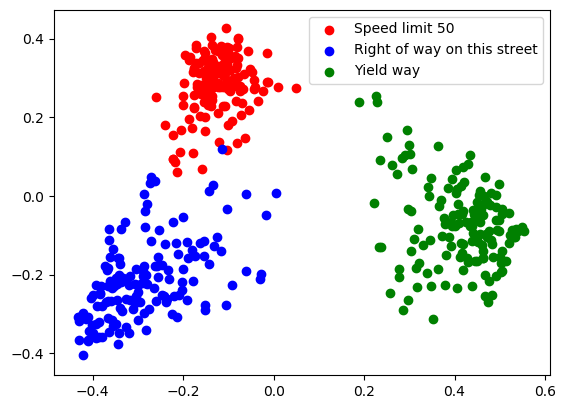
\includegraphics[scale=0.75]{./bilder/3_classes_pca.png}
\caption{Darstellung der Klassen nach der PCA-Transformation im 2D-Raum}
\end{figure}

Der Grafik kann man nun Nachbarschaftsbeziehungen der einzelnen Punkte, sowie auch Klassen entnehmen.
Daraus kann nun geschlussfolgert werden, dass der HOG-Deskriptor für die drei gewählten Klassen eine sehr gute Abgrenzung der Klassen generieren kann. Wie der Grafik zu entnehmen ist, ist diese Abgrenzung beinahe linear separierbar, was ein sehr wünschenswerter Fall ist, da dann die Algorithmen im folgenden leichter zu einer sehr guten Lösung kommen werden.\\

Unsere verwendete Klassifikationsmethode ist die Support-Vector-Machien (SVM). 
Vor dem Einsatz der SVM haben wir den Bestehenden Datensatz in 50\% Trainings-, 20\% Validation- und 30\% Test-Set aufgeteilt. Diese Aufteilung muss ausgeführt werden, da Supervised Learning Algorithmen in der Regel Hyperparameter besitzen. Dessen Werte müssen bestimmt werden und erfordern ein Verfahren um verschiedene Ausprägungen gegeneinander zu testen und die beste gefundene Alternative auszuwählen. Dieser Vergleich der Hyperparmater wird anhand der Auswertung des Validations-Sets ausgeführt und die Wahl der Hyperparameter-Ausprägungen und -Kombinationen haben wir mit der GridSearch ausgeführt.\\

Das Training und die Auswertung für den Datensatz mit den drei gewählten Klassen war wie zu erwarten zufriedenstellend und lieferte eine Genauigkeit von 100\%.
Die komplexere Problemstellung folgte aber darauf. Denn nun haben wir alle 43 gegebenen Klassen verwendet. Die folgende Abbildung soll den eben genannten Arbeitsablauf abbilden.\\

\begin{figure}[h]
\centering
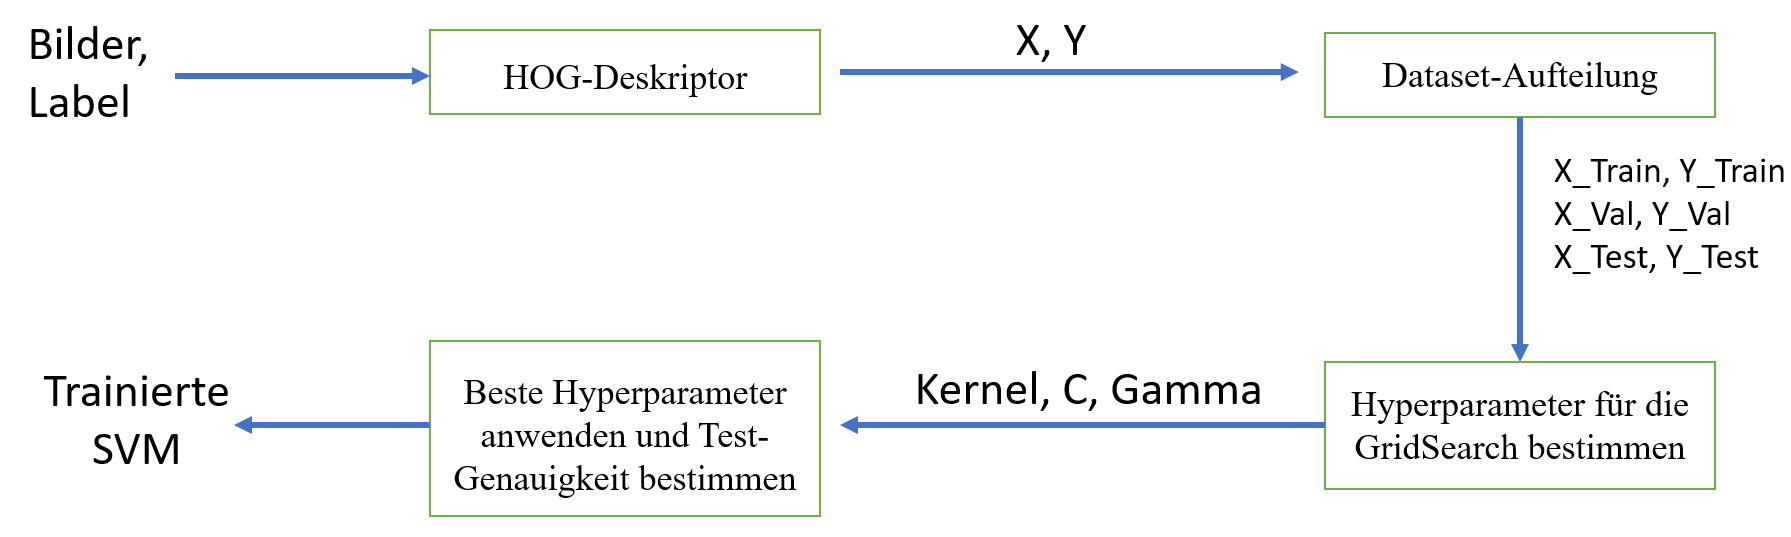
\includegraphics[scale=0.5]{./bilder/workflow.png}
\caption{Arbeitsablauf mit dem Datensatz zur Klassifikation}
\end{figure}

Nach Auswahl verschiedener Hyperparameter-Ausprägungen und Anwendung der GridSearch mit 10-Folds. Lieferte folgende Paramter-Konbination die beste Validation-Genauigkeit.
Kenrel: RBV, Gamma: 1.0 und C: 10.
Die resultierende Test-Genauigkeit beträgt 95\%.\\

Abschließend kann gesagt werden, die Kombination eines HOG-Deskriptor und der SVM liefter eine akzeptable Performance auf dem Dataset.
\chapter{Aufgaben von Tag 3}

Aufgaben von Tag 3
\chapter{Aufgaben von Tag 4}

Aufgaben von Tag 4
Abschluss
%%%%%%%%%%%%%%%%%%%%%%%%%%%%%%%%%%%%%%%%%%%%%%%%%%%%%
%%%%%%%%%         Ende der Kapitel         %%%%%%%%%%
%%%%%%%%%%%%%%%%%%%%%%%%%%%%%%%%%%%%%%%%%%%%%%%%%%%%%
\appendix 
\addcontentsline{toc}{chapter}{Anhang} 
\addtocontents{toc}{% 
  \protect\addtokomafont{chapterentry}{Anhang\ } 
} 
\chapter*{Anhang A. ...} 

...

\newpage
% Fügt das Literaturverzeichnis ein.
% Generell für das Zitieren bitte nur die literatur.bib Datei ändern.
% Zitieren: \footcite[Vgl. ][]{KEY}
\printbibliography
\end{document}